\section{Architecture}
Our System architecture -- shown in \autoref{fig:Giraf_comp_pic} has been designed with simplicity in mind and was greatly inspired by the MVC pattern. This means that the architecture is divided into three layers. The lowest layer is the database where the information is stored. Above this layer is the controller layer which, in the GIRAF platform, is known as Oasis. The controller is responsible for querying the database for information needed in an app and the controller is also responsible for storing information in the database. The last layer is the apps. This division of layers give the GIRAF platform a low cohesion which makes it easier to work with individual parts of the platform independently.

We have chosen to redesign last year's architecture \cite{LastYearsArchitecture} to make it easier to work with. We have simplified the architecture because we feel it is unnecessarily complex.

\begin{figure}
	\centering
		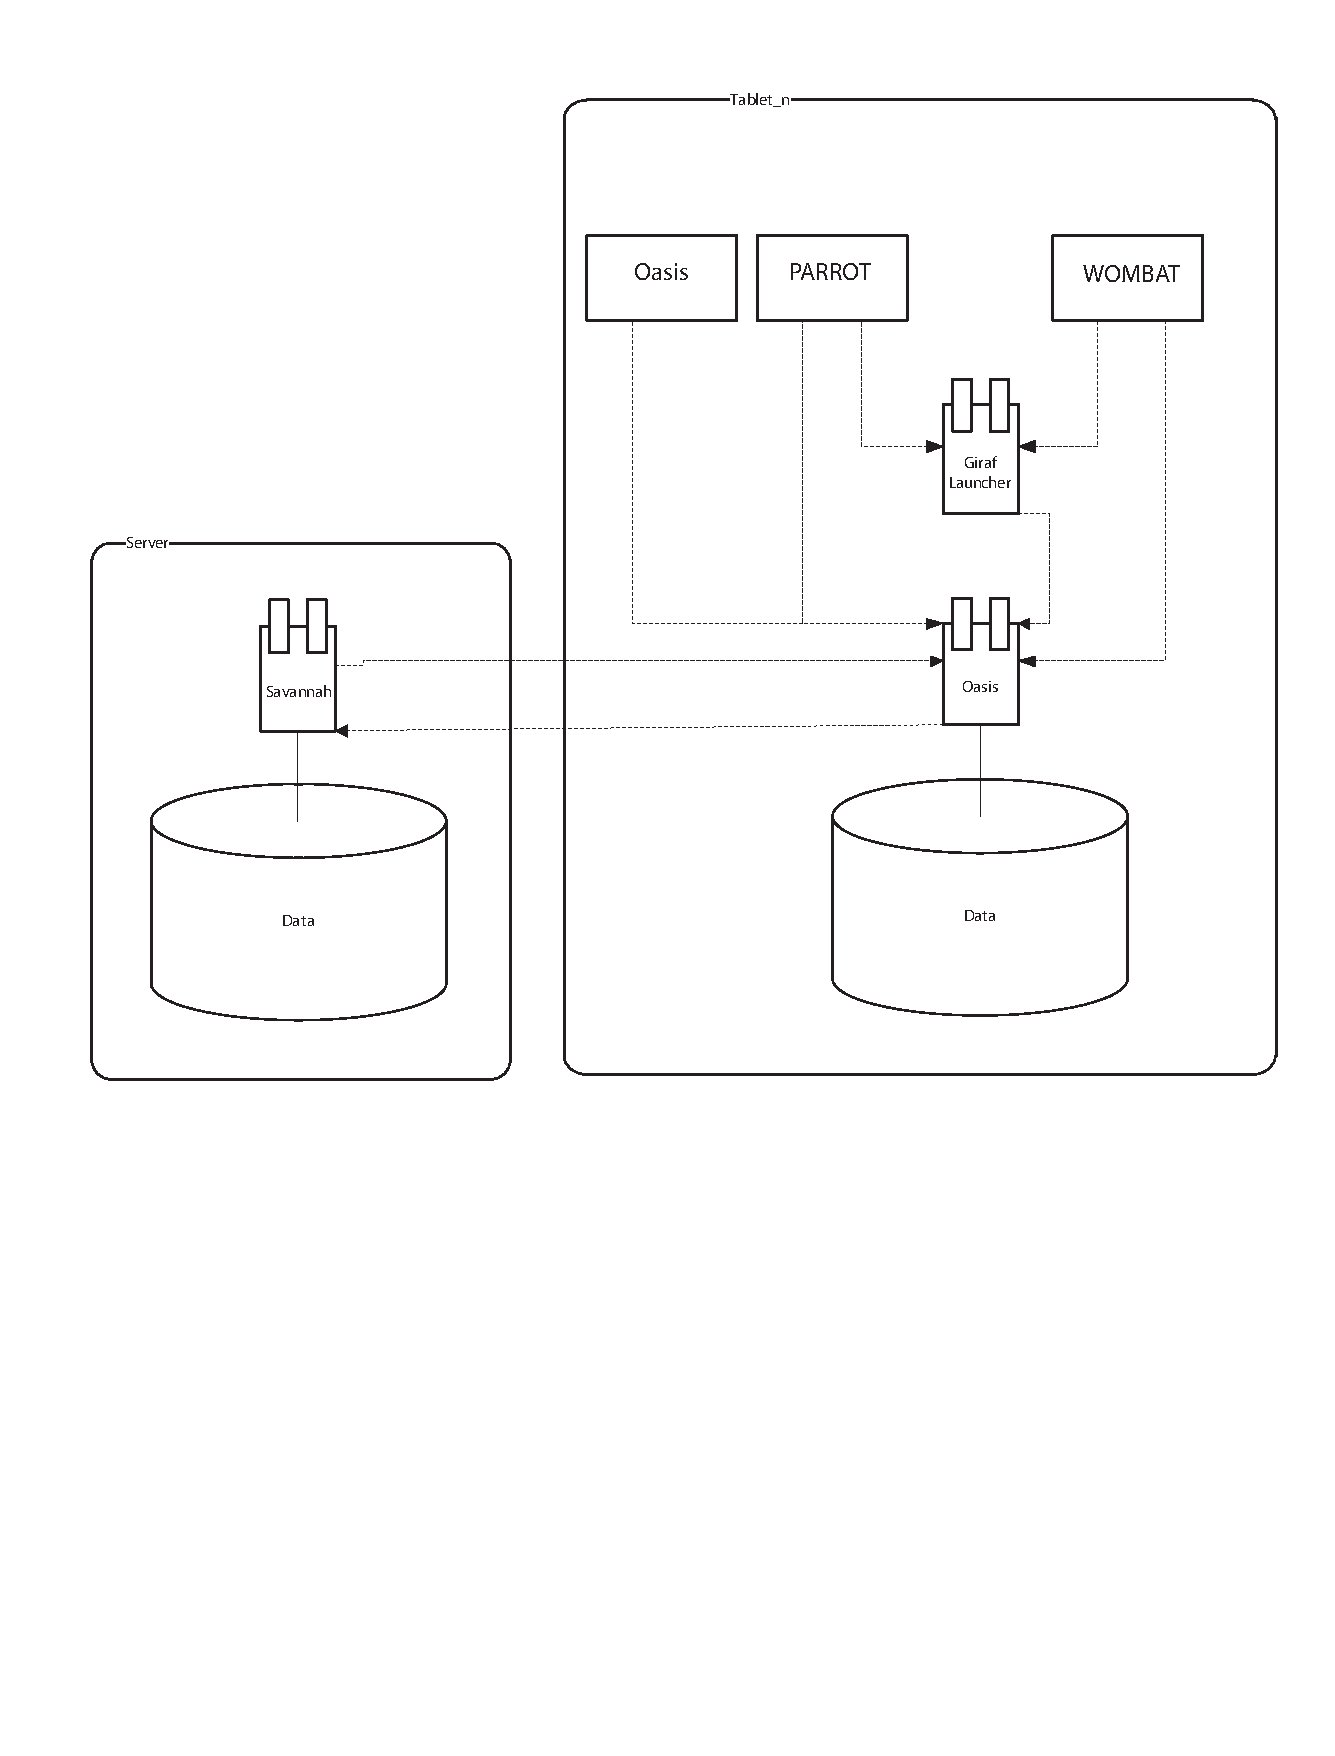
\includegraphics[width=\textwidth]{gfx/Giraf_comp.pdf}
	\caption{The GIRAF architecture}
	\label{fig:Giraf_comp_pic}
\end{figure}
